\begin{landscape}
\subsection{Zeit}	
    \begin{figure}[h!]
        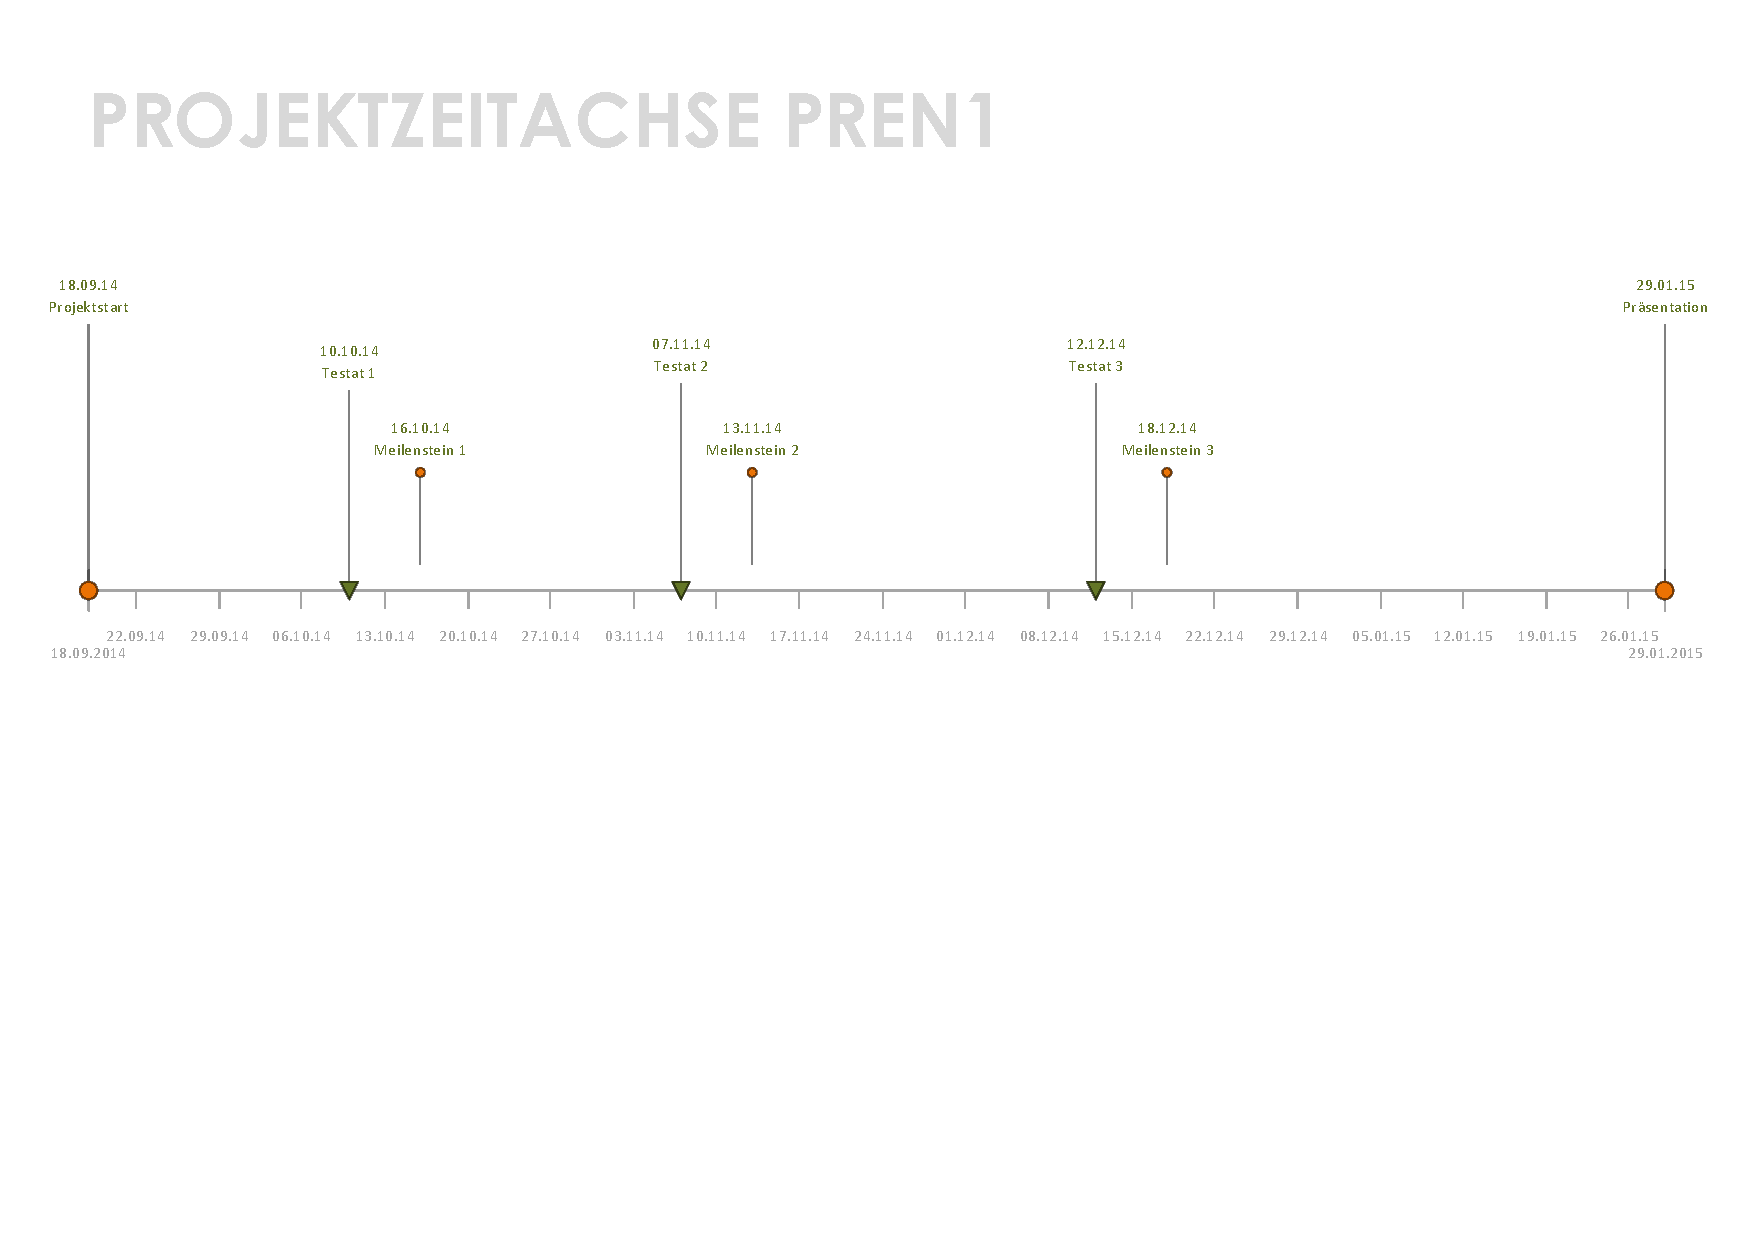
\includegraphics[page=1,scale=0.88,clip,trim=7mm 90mm 31mm 39mm] {Enddokumentation/Projektplanung_Management/Bilder/Projektzeitachse.pdf}
        \centering
        \caption{Zeitplan des Projekts} 
        \label{abb:ProjektZeitstrahl}
    \end{figure}
    
    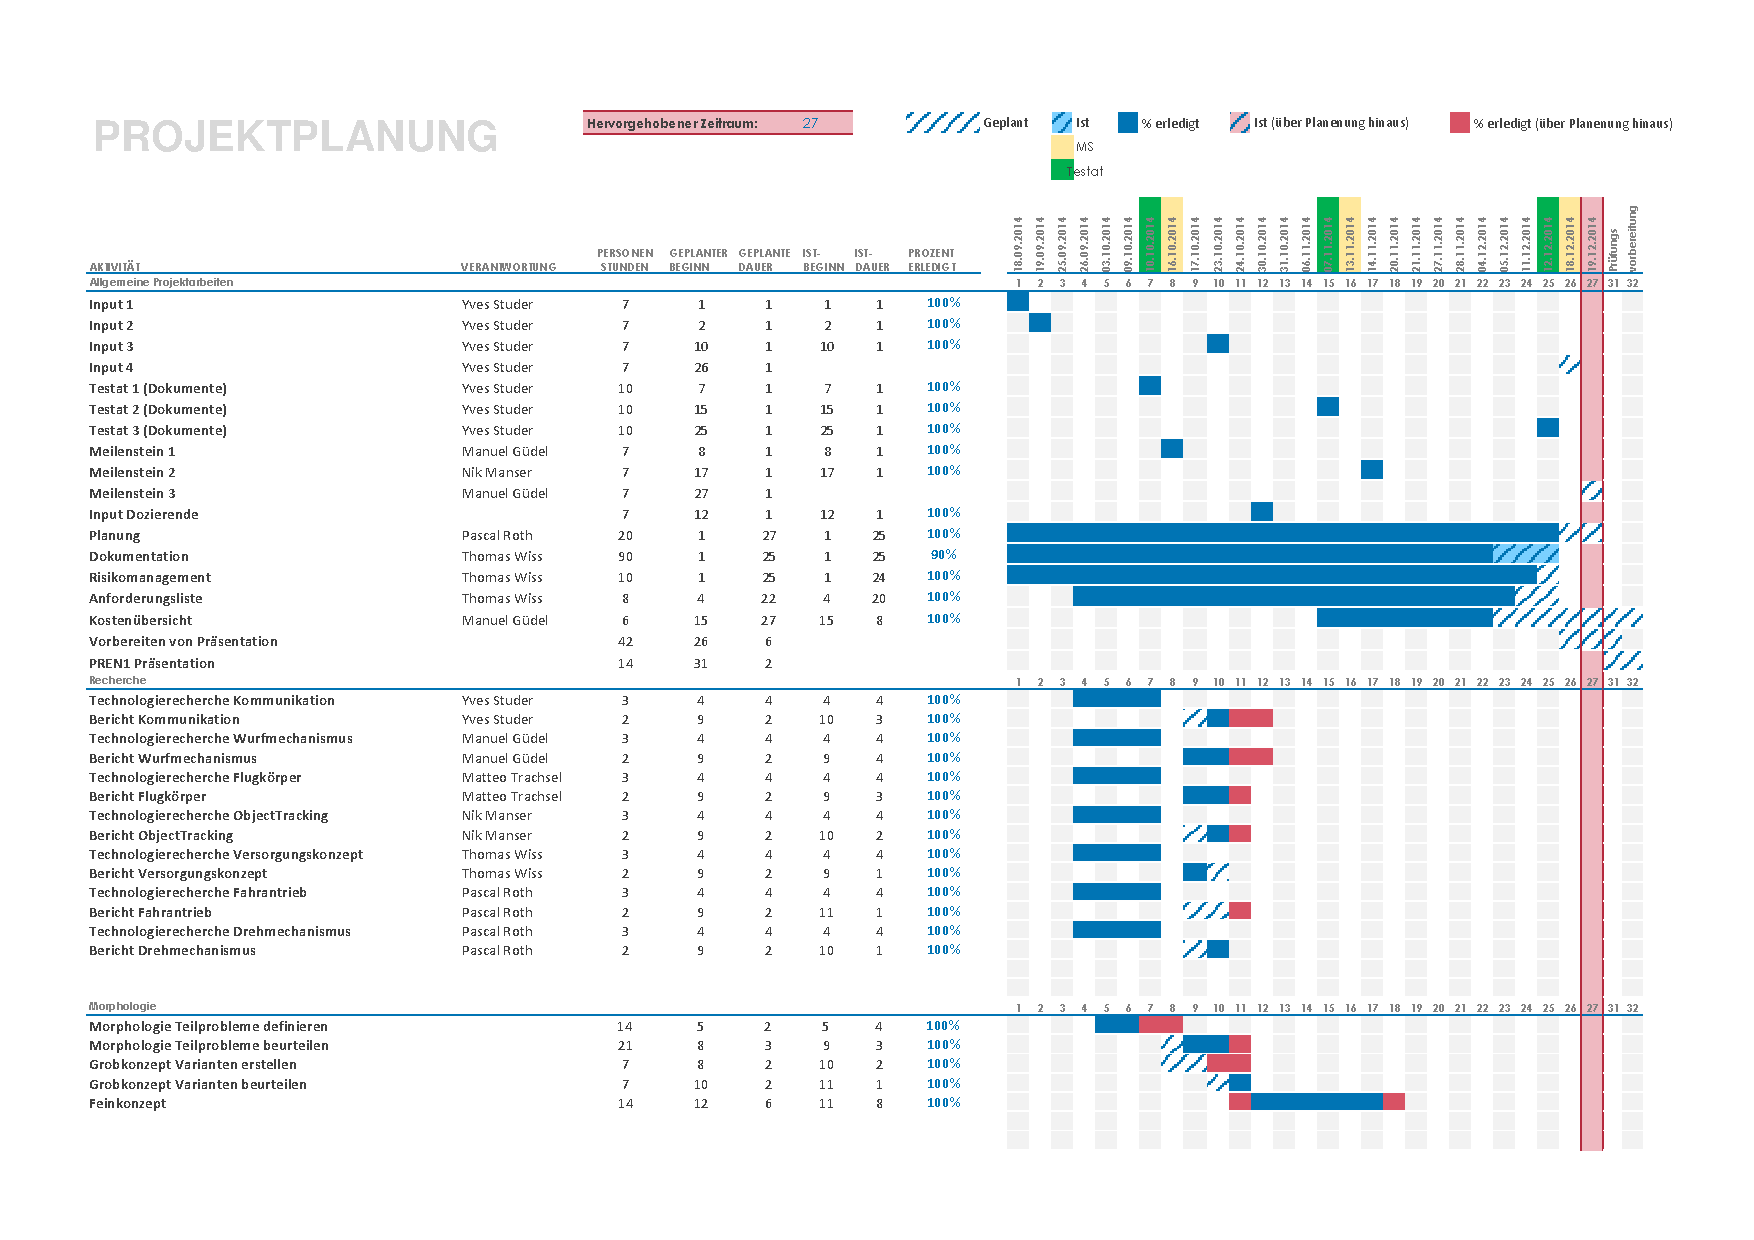
\includegraphics[page=1,scale=0.87,clip,trim=15mm 22mm 13mm 18mm] {Enddokumentation/Projektplanung_Management/Bilder/Projekt-Planung_Team32.pdf}
    \newpage
    \includegraphics[page=2,scale=0.87,clip,trim=15mm 100mm 13mm 10mm] {Enddokumentation/Projektplanung_Management/Bilder/Projekt-Planung_Team32.pdf}
\end{landscape}
%
\subsubsection{Erläuterung zur Projektplanung}
Um eine grösstmögliche Übersicht zu haben, ist die Projektplanung relativ 
allgemein gehalten. Das heisst, es sind alle Themen und Arbeitsblöcke vorhanden, 
jedoch ist nicht jeder einzelne Arbeitsschritt der darin anfällt auch aufgeführt. 
Ebenso ist pro Arbeitsschritt nur die verantwortliche Person aufgeführt. Sie 
trägt die Hauptverantwortung über ein Arbeitsblock, jedoch können auch andere 
Personen daran mitarbeiten. Abgeschlossene und nicht mehr relevante Arbeiten 
sind nicht aufgeführt. Zeitangaben sind als Schätzungen zu verstehen. Es wurde 
kein Journal über die geleistete Arbeitszeit geführt. Die auf den vorherigen 
Seite dargestellte Grafik ist die Projektplanung über den Zeitraum von PREN 1. 
Arbeiten, die noch nicht fertig sind oder die über den ganzen Zeitraum des 
PREN-Moduls laufen, werden Ende PREN 1 in eine neue Projektplanung für PREN 2 
überführt. Für diese Planung wird wiederum die selbe Excel-Vorlage verwendet. 
%
\subsubsection{Soll/Ist Zeitvergleich}
Die Zeiten welche in der Projektplanung angegeben sind, sind als Schätzungen 
zu betrachten, welche jeweils zu Beginn des Arbeitsblockes durch die 
verantwortliche Person gemacht wurde. Arbeitszeitrapporte oder Stundenblätter wurden 
nicht geführt. Dadurch kann die effektiv an einem Arbeitsblock gearbeitete Zeit 
abweichen. Vor allem den Administrativen Arbeiten und dem Dokumentieren wurde 
zu wenig Zeit zugesprochen. Dies zeigte sich jeweils beim Abschluss eines 
solchen Teilbereichs. Layout, Korrekturlesen, Änderungen etc. brauchten im 
Endeffekt fast immer mehr Zeit als veranschlagt. Dies ist ein wichtiger Punkt 
den es in der Zeitplanung im Hinblick auf PREN 2 zu beachten gilt. Die grösste 
Abweichung von der Planung gibt es sicherlich bei der Dokumentation. Hier wurde 
der Aufwand deutlich unterschätzt. Mit allen Formatierungs- und Layoutarbeiten 
ist schlussendlich zirka die doppelte Zeit dafür aufgewendet worden. Andere 
Arbeiten wie z.B. die Testversuche konnten gut im dafür vorgesehenen Zeitrahmen 
abgeschlossen werden. Über alles gesehen wird der Aufwand um ca. einen Viertel 
grösser sein als die Schätzung. In PREN 2 wird voraussichtlich jedes Teammitglied über seinen Arbeitsaufwand Buch führen, was eine genauere Kontrolle ermöglicht. Zudem ist geplant, vor allem dem Dokumentieren beim Schätzen mehr Pufferzeit zuzusprechen.